\chapter{Background}
\label{chap:background}

This chapter provides provides background information on the topics relevant to this thesis, pointing out to resources for further reading.
It introduces the concepts of artificial neural networks, different machine learning problem classes and learning paradigms, evolutionary algorithms, and neuroevolution.

\section{Artificial Neural Networks}

Artificial neural networks (ANNs) are a class of machine learning models, which are inspired by biological neural networks. ANNs are composed of interconnected
neurons, which are organized in layers. The first layer of an ANN is referred to as the input layer, the last layer as the output layer, and the layers
in between as hidden layers. In feed-forward ANNs, nodes in a layer are connected to nodes from the immediately preceding and succeeding layers. The connections between nodes
are associated weights, which are real-valued parameters.
Signal travels from the input layer to the output layer and the output of any node in the network is computed by applying a non-linear activation function
to the weighted sum of the inputs to the node as well as a bias term.
The weights of connections are typically learned using gradient-based optimization algorithms, such as backpropagation \cite{backpropagation}.

Given a neuron with inputs $x_1, x_2, \ldots, x_n$, bias $b$ and weights $w_1, w_2, \ldots, w_n$, the output $y$ of the neuron is computed as

\[
    y = f(b + \sum_{i=1}^{n} w_i x_i)
\]

where $f$ is the neuron's activation function.

An example of a feed-forward neural network is shown in \Cref{fig:ann}. This network consists of an input layer with four nodes, a hidden layer with five nodes,
and an output layer with one node. The connections between nodes are represented by arrows. Connection weights, biases and activation functions are
not shown. The network is fully connected, meaning that each node in a layer is connected to each node in the next layer.

\def\layersep{2.5cm}

\begin{figure}
    \begin{center}
        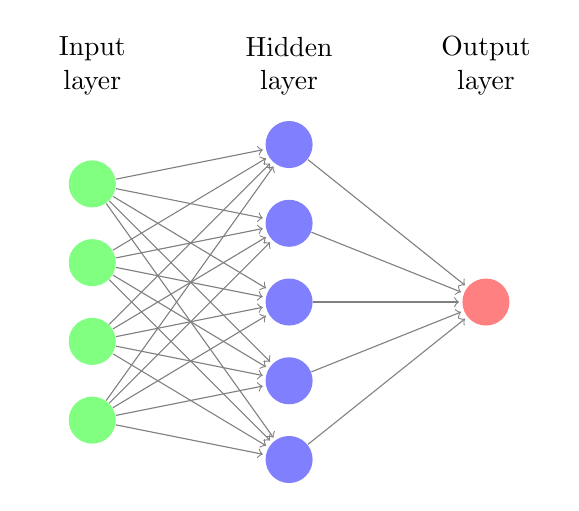
\begin{tikzpicture}[shorten >=1pt,->,draw=black!50, node distance=\layersep]
            \tikzstyle{every pin edge}=[<-,shorten <=1pt]
            \tikzstyle{neuron}=[circle,fill=black!25,minimum size=17pt,inner sep=0pt]
            \tikzstyle{input neuron}=[neuron, fill=green!50];
            \tikzstyle{output neuron}=[neuron, fill=red!50];
            \tikzstyle{hidden neuron}=[neuron, fill=blue!50];
            \tikzstyle{annot} = [text width=4em, text centered]

            % Draw the input layer nodes
            \foreach \name / \y in {1,...,4}
            % This is the same as writing \foreach \name / \y in {1/1,2/2,3/3,4/4}
                % \node[input neuron, pin=left:Input \#\y] (I-\name) at (0,-\y) {};
                \node[input neuron] (I-\name) at (0,-\y) {};

            % Draw the hidden layer nodes
            \foreach \name / \y in {1,...,5}
                \path[yshift=0.5cm]
                    node[hidden neuron] (H-\name) at (\layersep,-\y cm) {};

            % Draw the output layer node
            \node[output neuron, right of=H-3] (O) {};

            % Connect every node in the input layer with every node in the
            % hidden layer.
            \foreach \source in {1,...,4}
                \foreach \dest in {1,...,5}
                    \path (I-\source) edge (H-\dest);

            % Connect every node in the hidden layer with the output layer
            \foreach \source in {1,...,5}
                \path (H-\source) edge (O);

            % Annotate the layers
            \node[annot,above of=H-1, node distance=1cm] (hl) {Hidden layer};
            \node[annot,left of=hl] {Input layer};
            \node[annot,right of=hl] {Output layer};
        \end{tikzpicture}
        \caption{Graph representation of an ANN with one hidden layer.}
        \label{fig:ann}
    \end{center}
\end{figure}

Activation functions \cite{activation} are used to introduce non-linearity in the model, which is important to enable the model to learn complex patterns in the data. Without
non-linear activation functions, the model would be limited to learning linear functions, which are not sufficient to model complex relationships in the data.
Two commonly used activation functions are the sigmoid function and the rectified linear unit (ReLU) function. The sigmoid function is defined as
$\sigma(x) = \frac{1}{1 + e^{-x}}$, it maps the input to the range $[0, 1]$, making it useful for binary classification tasks. The ReLU function is defined as
$f(x) = \max(0, x)$, which is a piecewise linear function that maps negative inputs to zero and positive inputs to the input itself. The ReLU function is
commonly used in deep learning models, as it has been shown to improve the convergence of the optimization algorithm in deep architectures, by addressing the
vanishing gradient problem \cite{relu}. Graphs of the sigmoid and ReLU activation functions are shown in \Cref{fig:activation_functions}.

\begin{figure}
    \begin{center}
        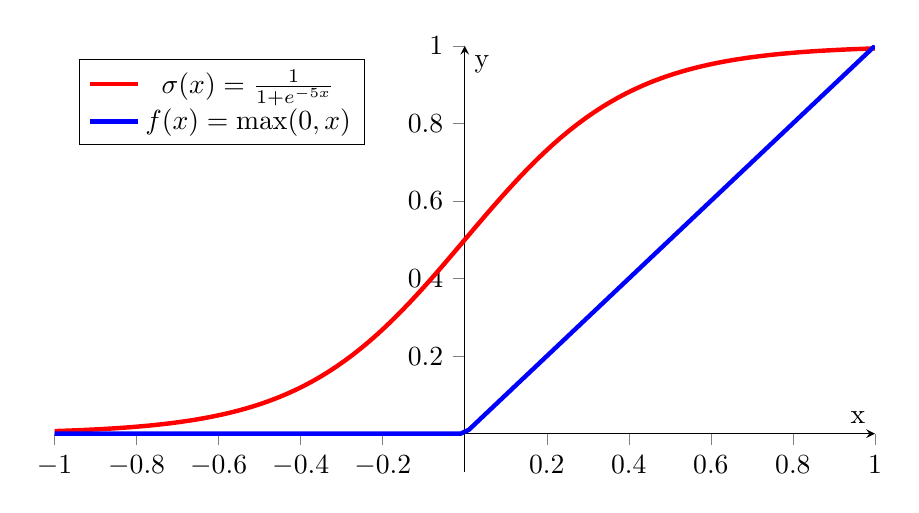
\begin{tikzpicture}
            \begin{axis}[
                axis lines=middle,
                width=12cm,
                height=7cm,
                tick align=outside,
                legend pos=north west,
                xmin=-1,
                xmax= 1,
                ymin= -0.1,
                ymax= 1,
                xlabel=x,
                ylabel=y]
                \addplot[domain=-1:1, red, ultra thick, samples=100] {1/(1+exp(-5*x))};
                \addplot[domain=-1:1, blue, ultra thick, samples=100] {max(0, x)};
                \addlegendentry{$\sigma(x) = \frac{1}{1 + e^{-5x}}$}
                \addlegendentry{$f(x) = \max(0, x)$}
            \end{axis}
        \end{tikzpicture}
        \caption{Graphs of the sigmoid and ReLU activation functions.}
        \label{fig:activation_functions}
    \end{center}
\end{figure}

Any continuous function can be approximated by ANNs \cite{approximation}. Over the years, these models have been applied to a wide range of problems, including classification and reinforcement
learning tasks. The process of applying ANNs consists in the design of its architecture, the choice of parameters such as the loss function or parameters for the
weigh optimization algorithm, and the optimization of its weights, in order to maximize its performance on a given task.

Many challenges are associated with the use of ANNs, such as the choice of the network architecture and hyperparameters, which can have an significant
impact on the performace of the model. Furthermore, the optimization of the network weights using gradient-based algorithms can result in various issues, such
as overfitting, which arises when the model performs well on the training data but poorly on unseen data, suboptimal local minima, and vanishing and
exploding gradients, when using deep networks \cite{overfitting,vanishing_gradient}.

\section{Problem classes and learning paradigms}

ANNs can be used to solve a wide range of problems, making use of different learning paradigms. This section provides a brief overview of the main classes of
problems and learning paradigms in machine learning.

\subsection{Supervised Learning}

Supervised learning is a class of machine learning tasks, where the goal is to learn a mapping from input data to output data, given a dataset of labeled
examples. The dataset consists of pairs of input-output data, and the goal is to learn a function which maps the input to the output. The function is typically
learned by minimizing a loss function \cite{on_loss,loss_survey}, which depends on the problem at hand, and which measures the difference between the predicted output and
the true output. The performance of the model is evaluated using a test set, which is separate from the training set. Supervised learning is used for tasks such
as classification and regression problems. For classification tasks, the output is a discrete class label, while for regression tasks, the output is a continuous value.
Famous examples of classification tasks include image classification \cite{cnn,cnn_survey}, where the goal is to classify images into different categories or spam detection \cite{spam_survey},
where the goal is to classify emails as spam or not spam. When two classes are involved, the task is referred to as binary classification.
Different metrics can be used to evaluate the performance of ANNs on classification tasks \cite{classification_metrics}, such as the accuracy which measures the proportion of correctly
classified examples. For regression tasks, metrics such as the mean squared error can be used.

\subsection{Unsupervised Learning}

Unsupervised learning \cite{unsupervised_learning} is a machine learning task where the goal is to learn patterns in the data without the use of labeled examples.
In other words, no ground-truth is provided from the (training) data and the goal is to learn the underlying structure of the data, such as clusters or a latent
representation space. Unsupervised learning is used for tasks such as clustering, which consists in grouping similar examples together, or dimensionality reduction
\cite{dimensionality_review,dimensionality_survey}, which consists in reducing the number of features in the data while preserving as much information as possible.

\subsection{Reinforcement Learning}

Reinforcement learning problems \cite{rl_survey} can be compared to trial-and-error learning. These problems are composed of three main components: an agent, an environment, and a reward
signal. The agent interacts with the environment by taking actions, and is provided with a reward signal which measures how well it is performing.. The agent interacts with
the environment by observing the current environment state, and taking actions. It receives a reward signal from the environment, the state is updated and the process is repeated.
As the agent interacts with the environment it learns a strategy mapping states to actions, which is referred to as a policy, with the goal of maximizing its cumulative reward.
Reinforcement learning is used for dynamic tasks such as game playing or control tasks.
There is no labeled data in reinforcement learning, and the agent must learn from its own experience, by exploring the environment and learning from the feedback it receives.

\section{Evolutionary Algorithms}

Evolutionary algorithms (EAs) are a class of optimization algorithms, which are inspired by the process of natural selection. EAs are based on the idea of
evolving a population of candidate solutions to a problem, in order to find the best solution. The process of evolution consists in the selection of the
fittest individuals, which are then recombined to produce offspring, which are then mutated. The fitness of the offspring is evaluated and the process is
repeated for a number of generations until a stopping criterion is met, such as a maximum number of generations, a maximum number of iterations with no improvement,
or a desired level of performance. At each generation, the population is updated by replacing the worst-performing individuals with the offspring.

Individuals are represented by genotypes, which are encoded in a way that allows the application of genetic operators, such as crossover and mutation, and
by phenotypes, which are the actual interpretation of the genotype used as solutions to the problem. The fitness of an individual is evaluated using a
fitness function, which measures the quality of the solution.

Mutations are used to introduce diversity in the population, which is important to avoid premature convergence to suboptimal solutions. During mutations,
parts of the genotype are modified while other parts remain unchanged, with the goal of performing a local search around the current genotype.
The individuals reproduce using crossover, which combines the genotypes of two parents to produce offspring. The offspring inherit parts of the genotypes
of the parents. The idea is that combining two good solutions should produce an even better solution.

The general structure of an evolutionary algorithm is shown in \Cref{alg:ea}.

\begin{algorithm}[H]
    \caption{General structure of an evolutionary algorithm.}
    \label{alg:ea}
    \begin{algorithmic}
        \State Initialize population
        \State Evaluate population
        \While{termination criterion not met}
            \State Select parents
            \State Recombine parents
            \State Mutate offspring
            \State Evaluate offspring
            \State Select survivors
        \EndWhile
        \State \textbf{return} best individual
    \end{algorithmic}
\end{algorithm}

It should be noted that evolutionary algorithms often have a variety of parameters that need to be tuned, such as the population size, the mutation rate,
the crossover rate, and the selection mechanism. The performance of the algorithm is sensitive to the choice of these parameters, and finding the
right combination of parameters can be a challenging task. For example, a mutation rate that is too low would result in a lack of diversity in the population, but if
it is too high, the algorithm might not converge to a high-quality solution, a trade-off that needs to be carefully balanced.

Evolutionary algorithms can be organized into different categories, including:

\begin{itemize}
    \item \textbf{Genetic algorithms (GAs):} Genetic Algorithms \cite{genetic_alg,genetic_alg_review} are generally applied to optimization problems and follow the principles described above.
    \item \textbf{Genetic programming (GP):} Genetic programming \cite{cartesian_gp} is a variant of genetic algorithms where the individuals are computer programs, which are evolved to
        solve a problem. Programs are traditionally represented as trees.
    \item \textbf{Evolution strategies (ES):} Evolution strategies \cite{es_intro} are black-box optimization algorithms, which are used to optimize continuous real-valued functions.
        Unlike other classes of EAs, evolution strategies do not maintain an explit population of individuals, but instead, a parametrized probability distribution
        used to sample the individuals.
\end{itemize}

\section{Neuroevolution}

Neuroevolution is a subfield of machine learning, which combines evolutionary algorithms and artificial neural networks. The idea is to evolve the weights,
and potentially, the architecture or hyperparameters of ANNs using an EA instead of gradient-based methods. Hence, this approach aims to
offer an alternative to the manual trial-and-error process of designing suited architectures and choosing hyperparameters. Furthermore, this approach,
being more general than traditional gradient-based methods, can be applied to a wide range of problems, without the need for any pre-defined knowledge on the task
at hand, such as reinforcement learning tasks, offering an alternative to the traditional reinforcement learning methods, which do not scale well for problems with large
state space or partial observability \cite{challenges_of_rl,rl_control}, or other problems where no training data is available to perform supervised learning.

However, neuroevolution generally comes with a major limitation which its computational cost, making it not suitable for the evolution of large networks,
while gradient-based methods have successfully been applied to networks with billions of parameters \cite{llama3}.
It is still particularly interesting for problems where smaller networks can be used or where other methods are not applicable.

From the perspective of the EA, neural networks serve as the phenotype, one of the main challenges is to define an encoding strategy into genotypes, which
allows for the conduction of genetic operations. For example, it is not trivial to define a crossover operation for neural networks when topologies are also
being evolved. For this reason, neuroevolution has traditionally  been used to evolve the weights of a fixed topology network. Genetic encoding strategies
for neural networks can be divided into two main categories:

\begin{itemize}
    \item \textbf{Direct encoding:} In the case of direct encodings \cite{neuroevolution_learning,neuroevolution_trends,neuroevolution_survey}, genomes contain the information for
        all nodes and connections in the network, and are directly translated into a network. This is the strategy which is employed by most neuroevolution algorithms.
    \item \textbf{Indirect encoding:} In the case of indirect encodings \cite{neuroevolution_learning,neuroevolution_trends,neuroevolution_survey}, Genomes contain a set of rules or
        instructions to generate the network, which is then constructed from these rules.
\end{itemize}

Neuroevolution algorithms evolving both the weights and the topology of the network are referred to as TWEANNs (Topology and Weight Evolving Artificial Neural Networks) \cite{neat}.
Lastly, neuroevolution can also be used in combination with traditional training methods to optimize the hyperparameters of a network, such as the learning rate or the
activation function, or the topology of the network, while the weights are learned using gradient-based methods \cite{neuroevolution_trends}.
